\documentclass[12pt,a4paper]{report}

% Packages
\usepackage[utf8]{inputenc}
\usepackage{graphicx}
\usepackage{hyperref}
\usepackage{setspace}
\usepackage{geometry}
\geometry{margin=1in}
\usepackage{tocloft} % for formatting TOC
\usepackage{titlesec} % for formatting headings
\usepackage{subcaption}
\usepackage{times}
\usepackage{xcolor}
\usepackage{booktabs}
\usepackage{float}
\usepackage{amsmath}
\usepackage{tabularx}
\usepackage{multirow}
\usepackage{listings}
\usepackage{pdfpages}

% Enable text wrapping and define style
\definecolor{codegreen}{rgb}{0,0.6,0}
\definecolor{codegray}{rgb}{0.5,0.5,0.5}
\definecolor{codepurple}{rgb}{0.58,0,0.82}
\definecolor{backcolour}{rgb}{0.95,0.95,0.92}

\lstdefinestyle{wrappedstyle}{
	backgroundcolor=\color{backcolour},   
	commentstyle=\color{codegreen},
	keywordstyle=\color{magenta},
	numberstyle=\tiny\color{codegray},
	stringstyle=\color{codepurple},
	basicstyle=\ttfamily\footnotesize,
	breakatwhitespace=false,         
	breaklines=true,                 % Enable line breaking
	breakautoindent=true,            % Maintain indentation on broken lines
	breakindent=0pt,                 % Indentation of broken lines
	postbreak=\space\space\space,    % Add spaces after break
	prebreak=\space,                 % Add space before break
	captionpos=b,                    
	keepspaces=true,                 
	numbers=left,                    
	numbersep=5pt,                  
	showspaces=false,                
	showstringspaces=false,
	showtabs=false,                  
	tabsize=2,
	frame=single,
	linewidth=\textwidth,            % Set line width to text width
	xleftmargin=0pt,                 % Remove left margin
	xrightmargin=0pt                 % Remove right margin
}

\lstset{style=wrappedstyle}

\usepackage[backend=biber,style=ieee]{biblatex}  % preamble
\addbibresource{references.bib} 
\DefineBibliographyStrings{english}{
	bibliography = {References},
}

% Force dotted leaders
\renewcommand{\cftchapdotsep}{\cftdotsep}
\renewcommand{\cftsecdotsep}{\cftdotsep}
\renewcommand{\cftsubsecdotsep}{\cftdotsep}

% Line spacing
% --- Page Setup ---
\geometry{
	a4paper,
	left=3cm,
	right=2cm,
	top=1.5cm,
	bottom=2.2cm
}

\onehalfspacing

% Start Here
\begin{document}
	
	\begin{titlepage}
		\centering
		\vspace*{0.2cm}
		\Large  {Project Synopsis Report} \\[0.1cm]
		\large on \\[0.1cm]
		\Huge \textbf{Project Title} \\[0.5cm]
		\large  {Submitted in partial fulfillment of the requirements of the degree of} \\[0.5cm]
		\Large \textbf{Bachelors of Engineering (B.E.)} \\[0.5cm]
		\large by \\[0.5cm]
		\large \textbf{Name of the Student } (UIN: \_\_\_\_\_) \\
		\large \textbf{Name of the Student } (UIN: \_\_\_\_\_) \\
		\large \textbf{Name of the Student } (UIN: \_\_\_\_\_) \\
		\large \textbf{Name of the Student } (UIN: \_\_\_\_\_) \\ [1cm]
		 
		
		\large {Guide:} \\ 
		\large \textbf{Name of Guide} \\[1cm]
		
		
\includegraphics[width=0.18\textwidth]{images/rcoe-logo.png}\\
		\Large \textbf{ Department of Computer Engineering} \\
		{\LARGE Rizvi College of Engineering} \\[1cm]
		
		
\includegraphics[width=0.15\textwidth]{images/mu-logo.png}\\
		\LARGE \textbf{University of Mumbai} \\
		2025--2026 \\
	\end{titlepage}
	
	% Certificate
	\chapter*{\centering \textit {Certificate}}
	This is to certify that the project synopsis entitled “Title of Project” has been submitted by Student Name 1, Student Name 2, Student Name 3 and Student Name 4 under the guidance of Prof. Guide Name in partial fulfillment of the requirement for the award of the Degree of Bachelor of Engineering in Computer Engineering from Rizvi College of Engineering, University of Mumbai.
	
	\vspace{2cm}
	\begin{flushleft}
	\begin{tabular}{p{10cm} p{10cm}}
		\underline{\hspace{5cm}} & \underline{\hspace{5cm}} \\
		Name of Guide & Prof. Mohd. Juned \\
		Project Guide & Head of Department \\
	\end{tabular}
	
	\vspace{1.5cm}
	\begin{tabular}{p{10cm} p{10cm}}
		\underline{\hspace{5cm}} & \underline{\hspace{5cm}} \\
		Internal Examiner & External Examiner \\
	\end{tabular}
	
	
	\vspace{1.5cm}
	\begin{tabular}{p{10cm} p{10cm}}
		\underline{\hspace{5cm}} & \underline{\hspace{5cm}} \\
		Assoc. Prof. Shiburaj Pappu & Dr. Varsha Shah \\
		Dean of Academics & Principal \\
	\end{tabular}

	\end{flushleft}
	
	\vspace{2cm}
	\begin{center}
	
\includegraphics[width=0.18\textwidth]{images/rcoe-logo.png}\\
	\large \textbf{Department of Computer Engineering} \\
	\Large \textbf{Rizvi College of Engineering} \\
	\normalsize {Off Carter Road, Bandra(W), Mumbai-400050.}
	\end{center}
	
	% Declaration
	\chapter*{Declaration}
	I declare that this written submission represents my ideas in my own words and where others' ideas or words have been included, I have adequately cited and referenced the original sources. I also declare that I have adhered to all principles of academic honesty and integrity and have not misrepresented or fabricated or falsified any idea/data/fact/source in my submission. I understand that any violation of the above will be cause for disciplinary action by the Institute and can also evoke penal action from the sources which have thus not been properly cited or from whom proper permission has not been taken when needed.
	
	\vspace{1cm}
	\begin{flushright}
		(Signature) \\[0.5cm]
		(Name of student and Roll No.) \\
		Date:
	\end{flushright}
	
	% Abstract
	\chapter*{Abstract}
	The 500-word abstract shall highlight the important features of the project report. \\
	Write your abstract here: description of work.
	
	\textbf{Keywords:} Keyword1, Keyword2, Keyword3
	
	% TOC
	\newpage
	\tableofcontents
	
	% Chapters
	\chapter{Introduction}
A brief explanation about the project topic is expected to be covered in this chapter (not more than 70-80 words).
	
\section{Background and Motivation}



\section{Problem Statement}



\section{Research Objectives}



\section{Scope and Limitations}
	
	\chapter{Review of Literature}
In this chapter include a critical appraisal of the previous work published in the literature pertaining to the topic of the investigation. Follow the below sample example.

\section{Review of Paper 1: Credit Card Fraud Detection Using Random Forest}


\subsection*{Methodology and Approach}
Smith et al. (2020) employed a Random Forest algorithm for credit card fraud detection, focusing on handling class imbalance through stratified sampling. Their approach involved feature engineering on transaction time, amount, and historical patterns.

\subsection*{Strengths and Contributions}
\begin{itemize}
\item Comprehensive feature engineering approach
\item Effective handling of class imbalance
\item High accuracy rates on benchmark dataset
\item Robust against overfitting
\end{itemize}

\subsection*{Limitations and Gaps}
\begin{itemize}
\item Computational intensity limits real-time application
\item Limited exploration of deep learning alternatives
\item Dataset restricted to European transactions only
\end{itemize}


	\chapter{Proposed System}
This chapter should discuss the details of the proposed system.
	

\section{Analysis/Framework/Algorithm}


\section{Details of Hardware \& Software}

\section{Design details}

\section{Methodology}

\section{Relevance to PO and PSO of the Department}




	
	\chapter{Implementation Plan and Status}
In this chapter explain the implementation plan and current status of the project along with Ghantt Chart.
	
\section{Latex Help}

\subsection{Tables in Latex}
The investigation utilized the publicly available Credit Card Fraud Detection dataset from Kaggle, containing transactions made by European cardholders in September 2013. Key dataset characteristics are summarized in Table \ref{tab:dataset_stats}.

\begin{table}[h!]
\centering
\caption{Dataset Characteristics and Statistics}
\label{tab:dataset_stats}
\begin{tabular}{lcc}
\toprule
\textbf{Parameter} & \textbf{Value} & \textbf{Percentage} \\
\midrule
Total Transactions & 284,807 & 100\% \\
Fraudulent Transactions & 492 & 0.172\% \\
Legitimate Transactions & 284,315 & 99.828\% \\
Features & 30 & - \\
Time Range & 2 days & - \\
\bottomrule
\end{tabular}
\end{table}

\subsection{Images in Latex}

The dataset contains 28 principal components obtained from PCA transformation, along with 'Time' and 'Amount' features. Figure \ref{fig:feature_dist} shows the distribution of selected features.

\begin{figure}[h!]
\centering
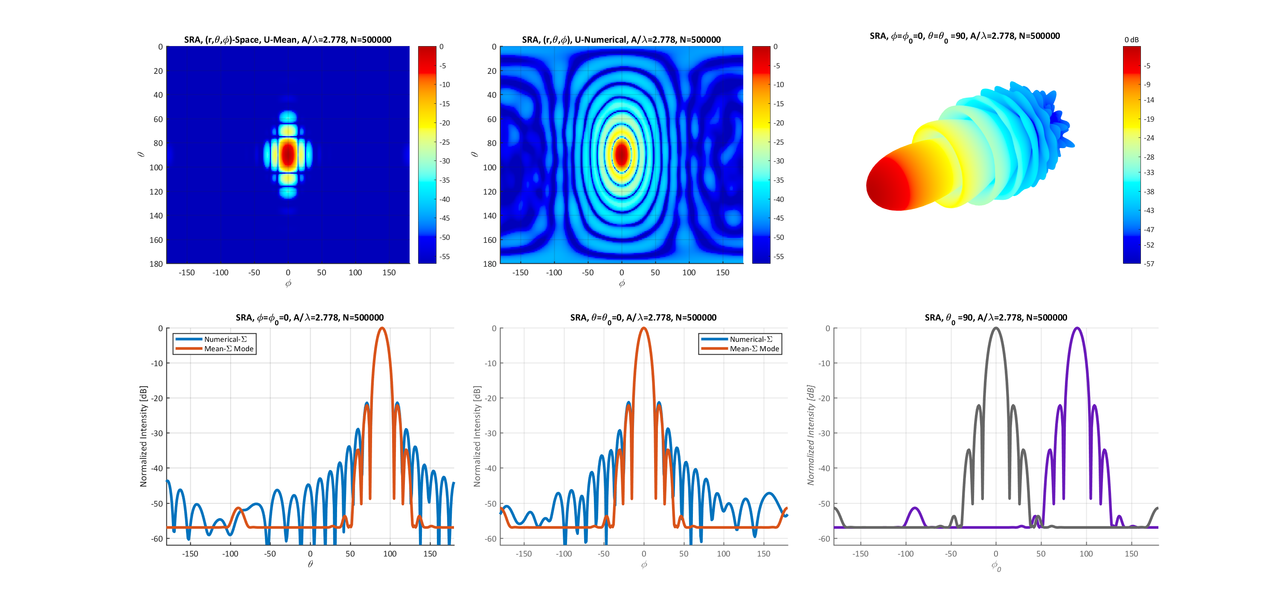
\includegraphics[width=0.8\textwidth]{images/feature_distribution.png}
\caption{Distribution of Features V1, V2, and Transaction Amount}
\label{fig:feature_dist}
\end{figure}



\subsection{List Items in Latex}

Three machine learning algorithms were implemented and compared:

\begin{itemize}
\item \textbf{Random Forest}: Ensemble learning method using multiple decision trees
\item \textbf{Logistic Regression}: Statistical model for binary classification
\item \textbf{Neural Network}: Deep learning approach with multiple hidden layers
\end{itemize}

Numbered:

\begin{enumerate}
	\item \textbf{Random Forest}: Ensemble learning method using multiple decision trees
	\item \textbf{Logistic Regression}: Statistical model for binary classification
	\item \textbf{Neural Network}: Deep learning approach with multiple hidden layers
\end{enumerate}

Nested List:

\begin{enumerate}
	\item Fruits
	\begin{itemize}
		\item Apple
		\item Banana
	\end{itemize}
	\item Vegetables
	\begin{itemize}
		\item Carrot
		\item Spinach
	\end{itemize}
\end{enumerate}


\subsection{Equations in Latex}

Sample Equationslike \eqref{eq:einstein} and \eqref{eq:einstein2}:

\begin{equation}
\text{Normalized Amount} = \frac{\text{Amount} - \mu_{\text{Amount}}}{\sigma_{\text{Amount}}}
\label{eq:einstein}
\end{equation}

\begin{equation}
\text{Time Feature} = \cos\left(2\pi \times \frac{\text{Time}}{86400}\right)
\label{eq:einstein2}
\end{equation}




\subsection{Include Graphics in PDF format}

You can include pdf diagrams for better clarity and printing \ref{fig:roc_curves}.

\begin{figure}[h!]
\centering
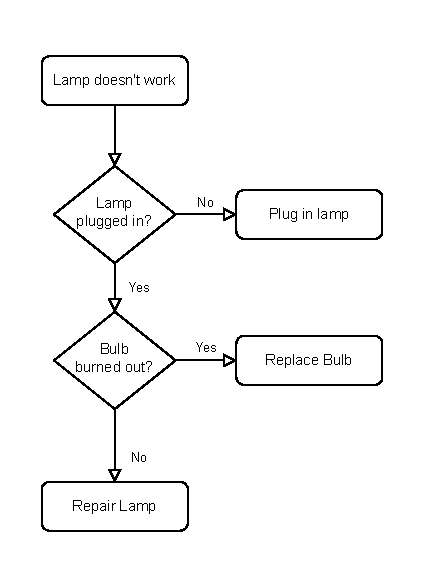
\includegraphics[width=0.8\textwidth]{images/flow.pdf}
\caption{ROC Curves Comparison of Implemented Algorithms}
\label{fig:roc_curves}
\end{figure}



	\chapter{Conclusions}
Conclusions derived from the logical analysis presented in the Results and Discussions Chapter shall be presented and clearly enumerated.
	
	
	\printbibliography

	\chapter*{Publications}
Please find the publication details of our paper.

\begin{itemize}
	\item \textbf{Title of Paper:} Title of our paper
	\item \textbf{Authors:} Name 1, Name 2, Name 3, Name 4, Prof. 
	\item \textbf{Journal/Conference Title:} Title of Journal or Conference
	\item \textbf{ISSN/ISBN Number:} 5655-6544
	\item \textbf{Link to Publication:} \url{https://www.example.com}
	
\end{itemize}

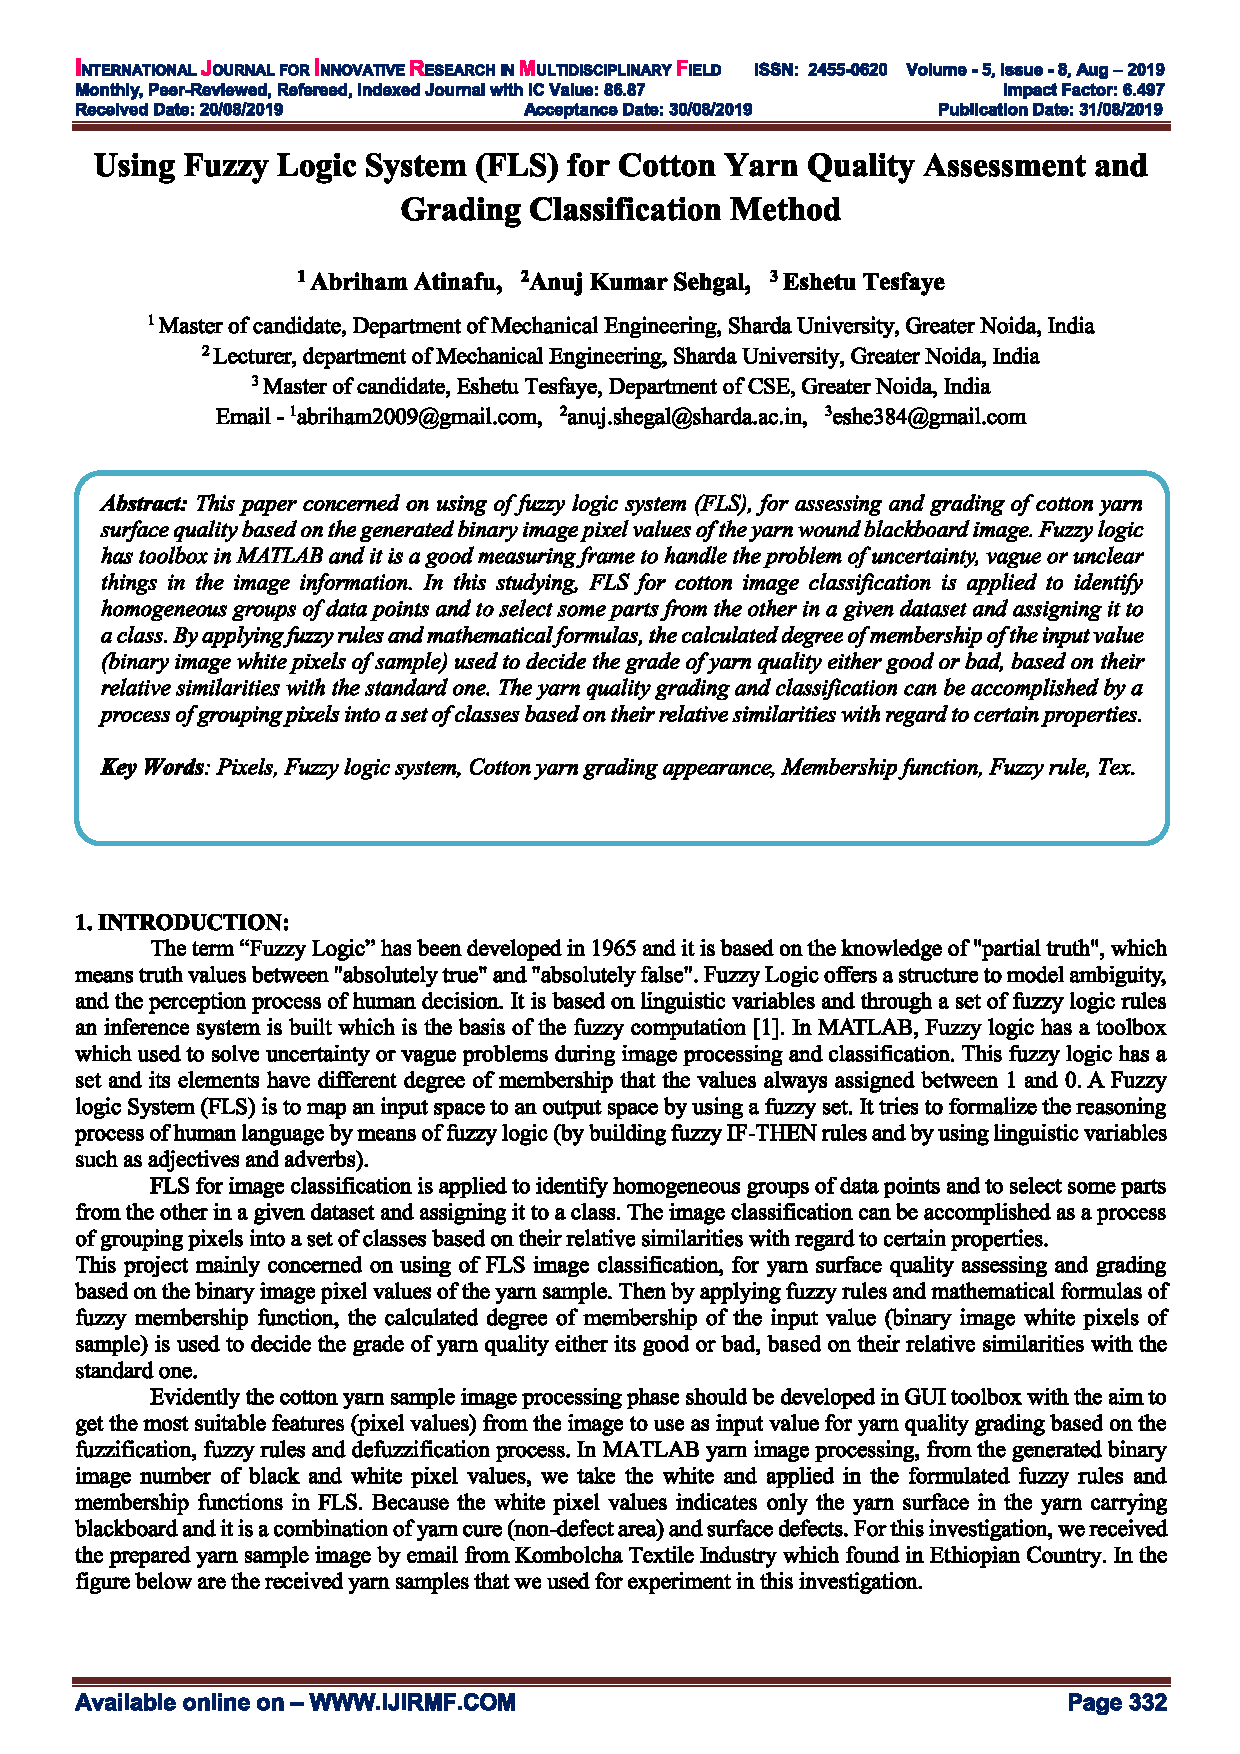
\includepdf[pages=-, scale=0.9, pagecommand={}]{my_publication.pdf}
	
\end{document}
